% rubber: depend ../../VERSION
\documentclass{frama-c-book}
\usepackage{amsmath}
\newcommand{\framacversion}%
           {\input{../../VERSION} (\input{../../VERSION_CODENAME}\unskip)}

\title{The Metrics plug-in}
\author{Richard Bonichon \& Boris Yakobowski}

\fcversion{\framacversion}

\cclicence{by-sa}
\copyrightstarts{2011}

\begin{document}
\sloppy
\emergencystretch 3em

\maketitle
\tableofcontents

\chapter{Quick overview}
\label{cha:quick-overview}

The Metrics plug-in computes complexity measures on C source code.
It can operate either on Frama-C's normalized abstract syntax tree  (AST) or on
the original source code.

\section{Description}
\label{sec:description}

\subsection{Command-line options}
\label{sec:cli-options}

The complete list of command-line options can be obtained by:
\begin{shell}
 % frama-c -metrics-help
\end{shell}

Let us now detail some of them:
\begin{description}
\item[-metrics] is a necessary switch to activate the plug-in. It also triggers
  the computation of syntactic metrics (slocs, number of statements
  of certain types, ...) on the normalized AST.

\item[-metrics-by-function] also computes (and displays) the above metrics, but
  this time on a per-function basis.

\item[-metrics-ast] is used to choose the AST the metrics should be computed
  on. It can be either Frama-C's normalized AST or the original AST. Section
  \ref{sec:metr-abstr-synt} covers this topic in some more details. How this
  affects the availability of metrics is discussed in Section
  \ref{sec:metr-norm-ast} and \ref{sec:metrics-original-ast}.

\item[-metrics-output] redirects metrics' calculations to a file. The selection
  of the output is automatically detected from the extension of the output
  file. As of now, only {\sf .html} or {\sf .txt} outputs are supported.

\item[-metrics-cover] specifies a set of functions from which to compute a
coverage estimate. This item is detailed in Section \ref{sec:eva-cover}.

\item[-metrics-eva-cover] activates the Eva coverage estimation.
  This item is detailed in Section \ref{sec:eva-cover}.

\item[-metrics-libc] controls whether functions from Frama-C's standard
  library are shown within the results. By default, this option is not set,
  and those functions are hidden.


\end{description}

\subsection{Metrics and abstract syntax trees}
\label{sec:metr-abstr-synt}
Frama-C analyses usually operate on its own internal {\em normalized} abstract syntax
tree\footnote{Note that the parsing machinery and the production of the abstract
  syntax trees originally come from CIL (\url{http://cil.sourceforge.net/}).}.
The normalization process
adds for example missing return statements, transforms all loops into while(1) \{ ... \}
statements, introduces some temporary variables...
Although this normalization process does not affect the semantic contents of the
code, its syntactic counterpart is indeed changed. It can therefore affect
metrics computed from the source code.

However, Frama-C also keeps the original abstract syntax tree of the source as
is. Even though Frama-C's analyses are usually centered around the normalized
representation, some facilities do exist to manipulate the other original AST.

Users of the Metrics plug-in can specify the nature of the AST from which the
metrics should be computed. Some metrics are available only for one AST
representation.

The default behavior, as enabled by the \verb+-metrics+ switch, is to calculate
syntactic metrics on the normalized AST. Metrics available for each AST are the
objects of Sections \ref{sec:metr-norm-ast} and \ref{sec:metrics-original-ast}.

\section{Metrics on the normalized abstract syntax tree}
\label{sec:metr-norm-ast}

\subsection{Syntactic metrics}
\label{sec:syntactic-metrics-normalized-ast}

Only cyclomatic numbers are available for the normalized AST. These are also
available through Frama-C's graphical user interface (GUI) (see Section
\ref{sec:gui}).

\def\pgname{reach.c}

Let us calculate the cyclomatic complexity of the program of Figure
\ref{fig:cprog} using the following command \footnote{{\sf frama-c -metrics
  -metrics-by-function -metrics-ast cil \pgname} is also a valid command for
this purpose. }.
\begin{shell}[escapechar={\#}]
% frama-c -metrics -metrics-by-function #\pgname#
\end{shell}
\begin{figure}
  \centering
  \lstinputlisting[language={[ANSI]C},alsolanguage=ACSL,style=frama-c-style,
  basicstyle=\lp@basic,firstline=5]
  {../../tests/metrics/\pgname}
  \caption{Source code for \pgname}
  \label{fig:cprog}
\end{figure}

The results are detailed in Figures~\ref{fig:cprog_output}
and~\ref{fig:cprog_output2}.
The output contains a summary, for each function, of the number
of assignments, function calls, exit points, declared functions (it should
always be 1), goto instructions, if statements, pointer dereferencings and lines
of code. The cyclomatic number of the function is also computed. Per-function
results are available only if the option {\sf -metrics-by-function} is
specified; otherwise only the ``Syntactic metrics'' part of the output is shown
(Figure~\ref{fig:cprog_output2}).
Note that these results can be printed to a text or html file using the {\sf
  -metrics-output} option.

\begin{figure}[!ht]
  \centering
  \lstinputlisting[language=Logs,basicstyle=\lp@basic, firstline = 3, lastline=48]{./cil.log}
  \caption{Output of by-function syntactic metrics for the normalized AST of \pgname}
  \label{fig:cprog_output}
\end{figure}

\begin{figure}[!ht]
  \centering
  \lstinputlisting[language=Logs,basicstyle=\lp@basic, firstline = 49]{./cil.log}
  \caption{Output of global syntactic metrics for the normalized AST of \pgname}
  \label{fig:cprog_output2}
\end{figure}

\subsection{Graphical User interface}
\label{sec:gui}

Metrics on the normalized AST are also accessible through Frama-C's
GUI. Cyclomatic complexity numbers are shown either globally on the left-hand
side pane of the GUI, after left-clicking the {\sf Measure} button (see
Figure~\ref{fig:gui_global}), or for a chosen function (see
Figure~\ref{fig:gui_function}). To access this functionality, you must
right-click on the line  where the function is defined to make a menu appear,
then left-click on {\sf Metrics} as shown in the figure.

\begin{figure}[!ht]
  \centering
  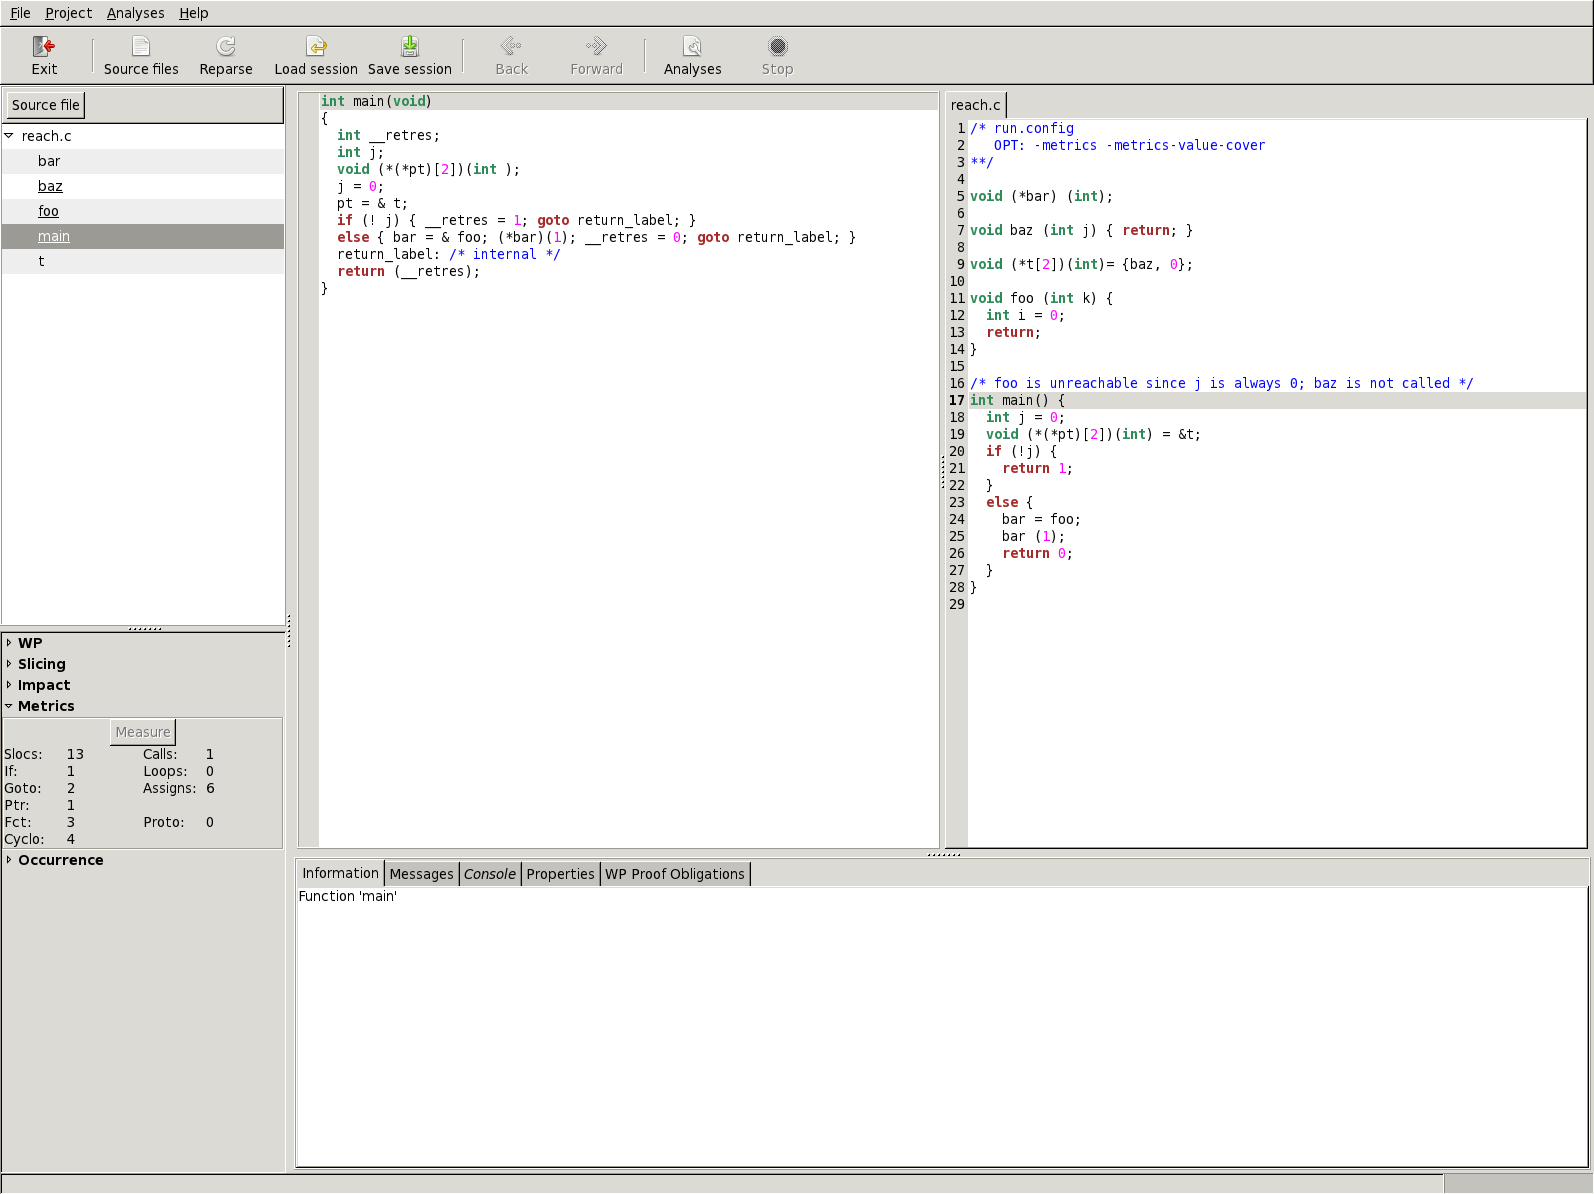
\includegraphics[width=\linewidth]{img/metrics_gui_global.png}
  \caption{Metrics GUI: calculate global metrics}
  \label{fig:gui_global}
\end{figure}

\begin{figure}[!ht]
  \centering
  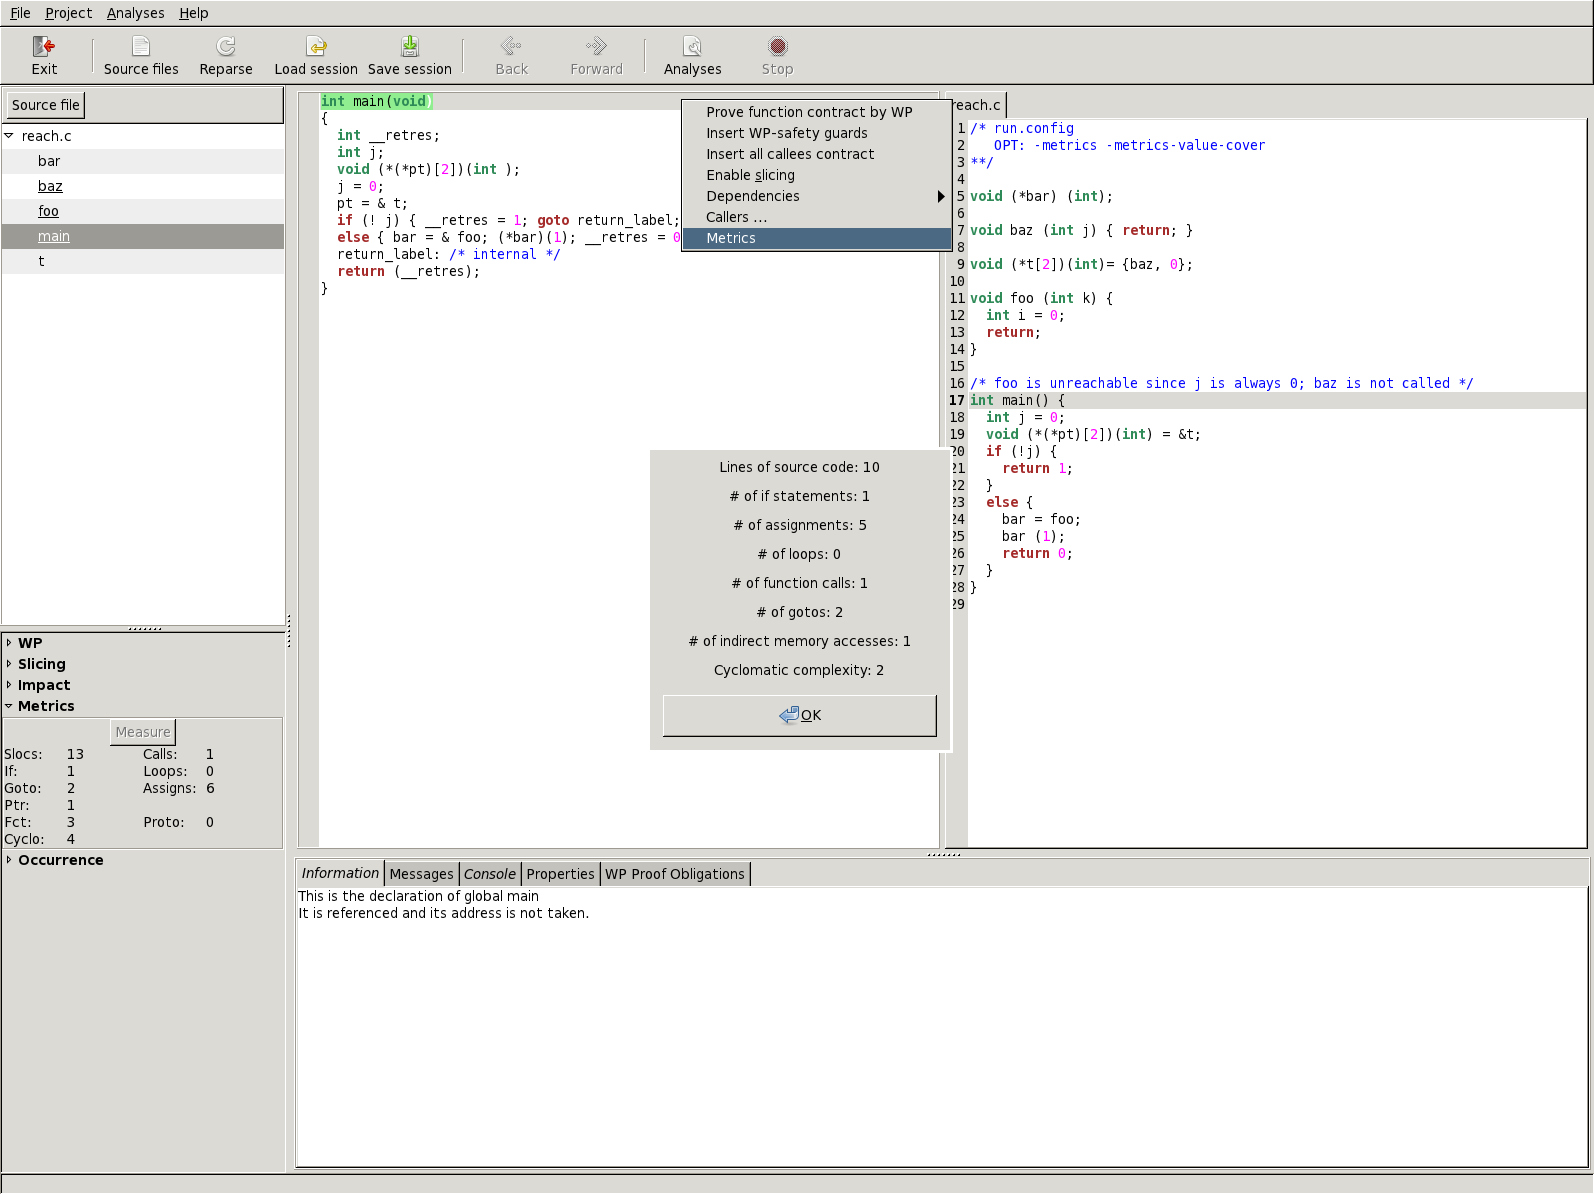
\includegraphics[width=\linewidth]{img/metrics_gui_function.png}
  \caption{Metrics GUI: calculate metrics for a function}
  \label{fig:gui_function}
\end{figure}


\subsection{Reachability coverage}
\label{sec:analysis-cover}

Given a function {\sf f}, the reachability coverage analysis over-approximates
the functions of the program that can be called from {\sf f}.
On our example, to activate it on the functions {\sf main} and {\sf foo},
one can use:
\begin{shell}[escapechar={\#}]
%  frama-c -metrics -metrics-cover main,foo #\pgname#
\end{shell}

The results are displayed in Figure \ref{fig:reach_cover}.
\begin{figure}[!ht]
  \centering
  \lstinputlisting[language=Logs, basicstyle=\lp@basic, firstline=33]{./reach.log}
  \caption{Reachability coverage for \pgname}
  \label{fig:reach_cover}
\end{figure}
The reachability coverage analysis is conservative. For example, it
considers that all function whose addresses are referenced within a
reachable function may be called. This explains why it considers that {\sf baz}
and {\sf foo} are reachable from the {\sf main} function.



\subsection{Eva coverage}
\label{sec:eva-cover}

The {\sf -metrics-eva-cover} option can be used to compare the code
effectively analyzed by Eva with what {\sf Metrics}
considers reachable from the {\sf main} function (wrt.\ the criterion
described in Section~\ref{sec:analysis-cover}).  The results of this option on our
example are given in Figure~\ref{fig:value-cover}. This particular
feature is activated by the following command:

\begin{shell}[escapechar={\#}]
%  frama-c -metrics -metrics-eva-cover #\pgname#
\end{shell}

Syntactic reachability is an over-approximation of what is actually
reachable by Eva. Thus, the coverage estimation will
always be equal to or less than $100\%$, especially if the source
code relies a lot on the use of function pointers.

For all functions that are considered syntactically reachable, but that
are not analyzed by Eva, the plug-in indicates the
locations in the code where a call \emph{might} have been analyzed.
In our example, this consists in the call to {\sf foo} at ligne 24.
Also, since the address of {\sf baz} is contained in
the initializer of the array {\sf t} (itself referenced in {\sf main}),
{\sf baz} is considered as callable; thus the plug-in signals the
initializer of {\sf t} as a possible calling point.
%
Finally, the plug-in displays the percentage of statements analyzed by Eva
for each function.

\begin{figure}[!ht]
  \centering
    \lstinputlisting[language=Logs, basicstyle=\lp@basic, firstline=42]{./cover.log}
  \caption{Eva coverage estimate for \pgname}
  \label{fig:value-cover}
\end{figure}


\section{Metrics on the original abstract syntax tree}
\label{sec:metrics-original-ast}

Only syntactic metrics are available on the original AST. Both Halstead and
cyclomatic complexity are computed. Note that this part of the plug-in
cannot be used through the GUI.

\begin{shell}[escapechar={\#}]
% frama-c -metrics -metrics-by-function -metrics-ast cabs #\pgname#
\end{shell}

\begin{figure}
  \centering
  \lstinputlisting[language=Logs,basicstyle=\lp@basic, firstline = 2, lastline=44]{./cabs.log}
  \caption{Cyclomatic metrics on the original AST for \pgname}
  \label{fig:cabs_metrics_cyclo}
\end{figure}

The effect is to calculate both cyclomatic and Halstead complexities for the
argument files, as shown in Figures~\ref{fig:cabs_metrics_cyclo} and
\ref{fig:cabs_metrics_halstead} . The results for
Halstead measures are only global while cyclomatic numbers can be done on a
per-function basis. Halstead measures also produce a detailed account
of the syntactic elements of the files.

\begin{figure}
  \centering
  \lstinputlisting[language=Logs,basicstyle=\lp@basic, firstline = 49]{./cabs.log}
  \caption{Halstead metrics on the original AST for \pgname}
  \label{fig:cabs_metrics_halstead}
\end{figure}


\chapter{Practical notes and comments}
\label{cha:pract-notes-comm}

\section{Cyclomatic complexity}
\label{sec:cycl-compl}

Cyclomatic complexity, also called conditional complexity was introduced by
Thomas \mbox{McCabe} \cite{DBLP:journals/tse/McCabe76} in 1976. It is a measure of the
number of paths through a source code and represent the complexity of the
control-flow of the program.

The cyclomatic number of a source code has been shown to be weakly correlated to
its number of defects.

\subsection{Calculation}

Cyclomatic complexity is a notion defined on a directed graph. It can therefore
be defined on a program taken as its control-flow graph. For a directed graph,
the cyclomatic complexity $C$ is defined as
\[ C = E - N - 2P \] where $E$ is the number of edges of the graph, $N$ the
number of nodes and $P$ the number of (strongly) connected components.

This notion of complexity is extended to deal with programs using the following
formula
\[ C = \pi - s + 2 \]
where $\pi$ is the number of decision points in the program
and $s$ the number of exit points.



\subsection{Practical notes}

Cyclomatic complexity can be computed on all abstract syntax trees in
Frama-C. The resulting complexity will nonetheless stay the same in both AST
representations, as Frama-C's normalized AST does not add control-flow
directives to the source code.

Prior to the computation of cyclomatic complexity, the plug-in gathers the
following syntactic information from the source code:
\begin{itemize}

\item Number of lines of code (assuming one C statement equals one line of code);
\item Number of if statements;
\item Number of loops;
\item Number of function calls;
\item Number of gotos;
\item Number of assignments;
\item Numbers of exit points (return statements);
\item Number of functions declared;
\item Number of pointer derefencings.
\item Number of decision points (conditional statements (if) and expressions
  (\verb|? :|), switch cases,
  lazy logical operators, loops).
\end{itemize}

These informations are computed both for the complete source code, and
on a per-function basis -- except for the number of functions
declared.

Cyclomatic complexity is then derived from these informations, both for the
full code and for each defined function.

\section{Halstead complexity}
\label{sec:halstead-complexity}
Halstead complexity is as set of software metrics introduce by Maurice Halstead
\cite{HalsteadComplexity} in 1977. The goal is to identify measurable properties
of the code and to go beyond pure complexity measures.

\subsection{Calculation}
\label{sec:halstead_computation}

Halstead complexity measures first need the following informations from the
source code:
\begin{itemize}
\item $\eta_{1}$ is the number of distinct operators;
\item $\eta_{2}$ is the number of distinct operands;
\item $N_{1}$ is the total number of operators;
\item $N_{2}$ is the total number of operands;
\end{itemize}

From the above informations, Halstead defines the following measures:
\begin{center}
  \begin{tabular}{lcl}
    Program vocabulary        &  $\eta$     & $\eta_{1} + \eta_{2}$ \\
    Program length            &  $N$       & $N_{1} + N_{2}$ \\
    Calculated program length &  $\hat{N}$
                              &  $n_{1} \times \text{log}_{2} \eta_{1} +
                                \eta_{2} \times \text{log}_{2}\eta_{2}$
                              \\
    Volume                    &  $V$        & $N \times \text{log}_{2} \eta$ \\
    Difficulty                &  $D$        & $(\eta_{1} / 2) \times N_{2} / \eta_{2}$ \\
    Effort                    &  $E$        & $D \times V $ \\
    Time required to program  &  $T$        & $E / 18$ \\
    Bugs                      &  $B$        & $E^{2/3} / 3000$ \\
  \end{tabular}
\end{center}

Note that ``Time required to program'' is an estimate given in seconds.

\subsection{Practical notes}
\label{sec:plug-functionalities}

To implement the measures defined in Section \ref{sec:halstead_computation}, it
is necessary to define what the operands and operators of the language are. For
Frama-C, the target language is C and we define its operands and operators as
follows:
\begin{description}
\item[Distinct operands] Identifiers and constants are operands, as well as type
  names and type specification keywords.
\item[Distinct operators] Storage class specifiers, type qualifiers, reserved
  keywords of C and other operators ($+, ++, +=$, ...) are considered as operators.
\end{description}

It is important to note that the measure of bugs delivered is considered
under-approximated for programs written in C.

\section{Eva coverage}

This part of the Metrics plug-in is thought of as a help for new code
exploration with Frama-C's Eva plug-in. The first steps into a new
code can
be quite complicated and, more often than not, Eva stops due to too
much imprecision. This imprecision can have a lot of different causes (body of
library functions missing, imprecisions of reads in memory, \ldots).

The graphical user interface helps visualizing where Eva has
stopped. The penetration estimate of Metrics aims to complement that by giving a
rough approximate of the percentage of code that Eva has
seen. This is especially interesting when comparing two runs of Eva
on the same code, after performing some tweaks and improvements to help
Eva: one can thusly quantify the added penetration due
to the tweaks.



\bibliographystyle{plain}
\bibliography{biblio}

\end{document}

%%% Local Variables:
%%% mode: latex
%%% TeX-master: "Makefile"
%%% End:
